\section{Análisis del algoritmo de Kruskal}
\frame{\sectionpage}

\begin{frame}[allowframebreaks]{Algoritmo de Kruskal}
    \begin{algorithm}[H]
        \caption{Algoritmo de Kruskal} \label{alg:kru}
        \begin{algorithmic}[1]
            \State $V \gets \texttt{list(vertices)}$
            \State $E \gets \texttt{list(aristasConPesos)}$
            \State $T = [ ]$
            \If{$ 0 \leq \texttt{len($E$)} \leq \texttt{len($V$)} \land \texttt{len($V$)} > 0$} \Comment{\textcolor{yellow}{Sacado de \cite{Albertson_Hutchinson_1988} que tiene que se V-1 y el paso 1 de \cite{Crisler_Froelich_Fisher_1999}}}
                \State return Error: no hay aristas o no está conectado
            \EndIf
            \algstore{kruskal}
        \end{algorithmic} 
    \end{algorithm}
    \begin{algorithm}[H]
        \begin{algorithmic}[1]
            \algrestore{kruskal}
            \State sort(E) \Comment{\textcolor{yellow}{ajusta para que los vertices estén ordenados acendientemente por peso, no explicitamente mencionado en todos los libros, pero \cite{Albertson_Hutchinson_1988} si lo toma en cuenta a la hora de hacer el cálculo de tiempo}}
            \For{$i \; \texttt{in} \; E$}
                \If{$! \texttt{find($i$, $T$)}$} \Comment{\textcolor{yellow}{busca que no haya i en T y que i no haya un ciclo con lo que ya está guardando en T}}
                    \State $\texttt{union($i$, $T$)}$ \Comment{\textcolor{yellow}{ingresa la arista i }}
                \EndIf
            \EndFor
        \end{algorithmic} 
    \end{algorithm}
\end{frame}

\begin{frame}[allowframebreaks]{Tiempo del algoritmo de Kruskal}
Aquí podemos asimilar varios análisis de diferentes fuentes. 
\begin{itemize}
    \item Primero \cite{Albertson_Hutchinson_1988} concluye que si el sorteo de las aristas no está optimizado puede llegar a ser \textcolor{yellow}{$O(E^2)$}. Las comparaciones (lo que están tomando como el find-union, o disjoint-set como lo conocen en otros libros, en este solo mencionan una unión y comparación) puede llegar a ser hasta \textcolor{yellow}{$O(V)$} comparaciones o a lo máximo \textcolor{yellow}{$O(EV)$}. Entonces que la complejidad de tiempo es de \textcolor{orange2}{$O(E^2 + EV)$} o con un algoritmo de sorteo eficiente \textcolor{orange2}{$O(E \log E)$} (E siendo el número de aristas y V siendo el número de vertices). Y por último menciona que \textcolor{yellow}{$E \leq V(V-1)/2 = O(V^2)$}
    \item Segundo tanto \cite{geeksforgeeksKruskal} como \cite{Dasgupta_Papadimitriou_Vazirani_2006} concluyen que sabiendo \textcolor{yellow}{$\log E \approx \log V$} el resultado es \textcolor{yellow}{$O(E\log E + E\log E)$} (uno el tiempo del sorteo el otro como el tiempo del union-find) o también se puede expresar como \textcolor{orange2}{$O(E\log E)$} (o \textcolor{orange2}{$O(E\log V)$})
    \item Tercero es importante notar que \cite{geeksforgeeksUnionFind} prueba que el algoritmo de union() y find() se puede hacer con fuerza bruta y da en el peor de los casos \textcolor{yellow}{$O(n)$ (lineal)}, verificando lo que dice la primera fuente que es el número de aristas * números de vertices
    \item Entonces para concluir como el curso es pesimista en su análisis el peor resultado es \textcolor{orange2}{$O(E^2) + O(EV) \sim O(E^2)$}, en vez de \textcolor{yellow}{$O(E\log E) + O(E\log E) \sim O(E \log E)$}
\end{itemize} \newpage

\centering
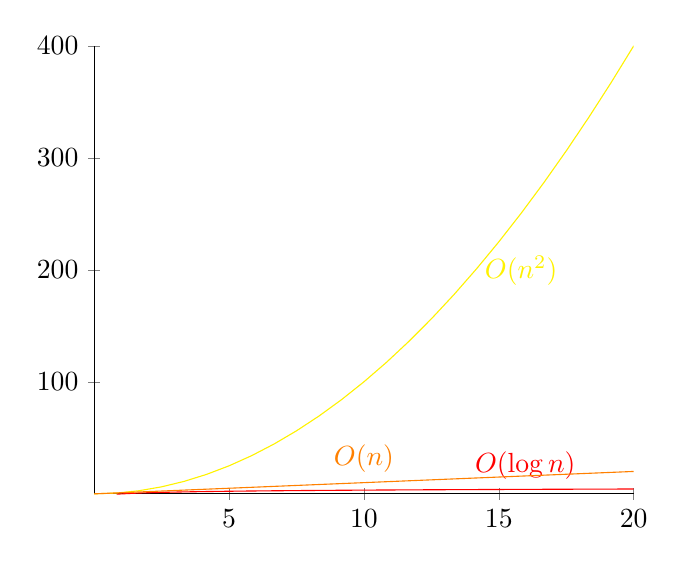
\begin{tikzpicture}
    \begin{axis} [domain=0:20, axis lines=middle, axis line style={-}]
        \addplot[color=yellow]{x^2} node[right,pos=0.5] {$O(n^2)$};
        \addplot[color=red]{log2(x)} node[above,pos=0.8] {$O(\log n)$};
        \addplot[color=orange]{x} node[above,pos=0.5] {$O(n)$};
    \end{axis}
\end{tikzpicture} \\
Prueba que $O(E^2)$ es el de mayor impacto \newpage

\begin{block}{Resumen de puntos importantes}
    Tiempo de sorteo pesimista: $O(E^2)$ \\
    Tiempo del find-union pesimista: $O(EV)$ \\
    Tiempo de Kruskal Pesimista: $O(E^2) + O(EV) \sim O(E^2)$ \\
    Tiempo de Kruskal optimizado: $O(E\log E) + O(E\log E) \sim O(E \log E)$
\end{block}
\end{frame}